\section{Funciones de activación}

Recordando que la forma de las funciones de activación es $y = f(x)$, donde $x$ representa el potencial postsináptico e $y$ el estado de activación de la neurona, es decir si va a lanzar un disparo o no. Las funciones de activación más empleadas son:

\begin{figure}[h]
    \centering
    \subfloat[Función logistica.]{
            \begin{tikzpicture}
            \begin{axis}[width=5.5cm,height=4cm,ylabel=$\sigma(z)$,xlabel=$z$,ymin=0,ymax=1.25,xmin=-5,xmax=5]
                \addplot[blue,smooth] {1/(1+exp(-x))};
                \addlegendentry{$y = \dfrac{1}{1+e^{-x}}$}
            \end{axis}
        \end{tikzpicture}
    }
    \subfloat[Función tangente hiperbólica.]{
        \begin{tikzpicture}
            \begin{axis}[width=5.5cm,height=4cm,ylabel=$\tanh(z)$,xlabel=$z$,ymin=-1.25,ymax=1.25,xmin=-5,xmax=5]
                \addplot[blue,smooth] {tanh(x)};
                \addlegendentry{$y = \dfrac{e^{x}-e^{-x}}{e^{x}+e^{-x}}$}
            \end{axis}
        \end{tikzpicture}
    }\\
    \subfloat[Función escalón.]{
            \begin{tikzpicture}
            \begin{axis}[width=5.5cm,height=4cm,ylabel=$\sigma(z)$,xlabel=$z$,ymin=-0.1,ymax=1.25,xmin=-1,xmax=1]
                \addlegendimage{ultra thick,blue}
                \addplot[ultra thick,blue,mark=*,mark options={fill=white},samples at={-1.1,0}] {0};
                \addplot[ultra thick,blue,mark=*,samples at={0,1.1}] {0.5};
                \addlegendentry{$y=\begin{cases} 1 \quad &\text{si} \, x \geq 0 \\ 0 \quad &\text{si} \, x < 0 \\ \end{cases}$
            }   
            \end{axis}
        \end{tikzpicture}
    }
    \subfloat[Función lineal a tramos. Tangente hiperbólica rectificada.]{
        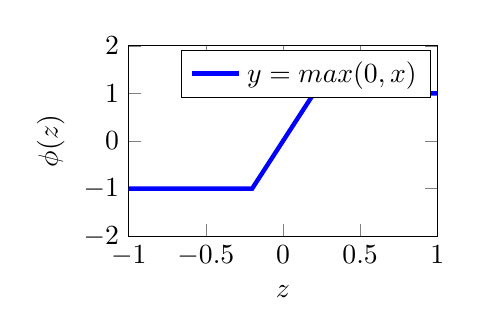
\begin{tikzpicture}
            \begin{axis}[width=5.5cm,height=4cm,ylabel=$\phi(z)$,xlabel=$z$,ymin=-2,ymax=2,xmin=-1,xmax=1]
                \addplot[blue,ultra thick] coordinates {(-1.1,-1) (-0.2,-1) (0.2,1) (1.1,1)};
                \addlegendentry{$y=max(0,x)$}
            \end{axis}
        \end{tikzpicture}
    }
        \caption[Funciones de activación sigmoides]{
        Las funciones de activación más usadas son la función sigmoide $\sigma(z)$ y la tangente hiperbólica $tanh(z)$.}
        \label{fig:sigmoid-tanh}
\end{figure}


